
\chapter{Solver selection and configuration}
\label{chapter:solver configuration}

% from numerical integration to system of linear equations
Numerical integration of time dependent partial differential equations can be achieved using different numerical schemes, namely: Runge-Kutta methods. In numerical analysis, the Runge–Kutta methods are a family of implicit and explicit iterative methods \cite{wiki:runge-kutta}.  \\


Implicit and explicit methods have their advantages and disadvantages which can be found in the corresponding literature.
% reference on something

 In general, implicit methods are robust in case of stiff equations, however, on another hand they are more expensive in terms of computational cost since they introduce a non-linear part that has to be solve using the Newton's method as an example. There is also a class of integration methods called semi-implicit that were designed to reduce the cost of implicit ones and be able to cope with stiff equations. But in all cases numerical integration boils down to solution of a couple systems of linear equations of a type:

\begin{equation} \label{eq:slq}
	Ax = b
\end{equation}

 where $A \in \mathbb{R^{N \times N}}$ is an invertible square matrix, $b \in \mathbb{R^{N}}$ represents the right-hand side, and $x \in \mathbb{R^{N}}$ is the solution vector. At this point we refer to a system of linear equations as just a system and we will use these two terms interchangeably. \\
 
In some cases, especially in case of implicit or semi-implicit methods, we have to compute several systems to perform one step of numerical integration. Thus, solution of a system \ref{eq:slq} is the computational core of any time integration scheme. In fact, it is the most expensive part and it is primary source of code optimization. \\ 

There are three major ways to solve a system of linear equations, namely: direct dense methods, sparse direct methods and iterative methods.\\

In the following sections \ref{subseq:direct methods}, \ref{subseq:iterative methods}, \ref{subseq:sparse methods} we are briefly going to review all three types of numerical solvers as well as their advantages and disadvantages and some aspects of their parallel implementations with a strong focus on their strong scaling behavior. Strong scaling is important for this research since we want to find a solver and its configuration to solve a certain system with a fixed size as fast as possible. Additionally to that, due to a large number of numerical integration steps, we want to find a robust solver to avoid any application crash during simulations.

At this point we can set requirements for a solver that we are looking for:

\begin{itemize}
	\item efficiency
	\item robustness
	\item numerical stability
	\item open source licenses
\end{itemize}

% TODO: observation of all possible methods to solve Ax = b. At this section you have to come to a conclusion that we have to use sparse direct methods


\section{Direct dense methods} \label{subseq:direct methods}

\todo{MUST BE ONLY 2D Scalapack EXAMPLE HERE}

Direct methods have very good numerical stability properties. They do not require to modify a system of equations as it is necessary for iterative methods. Sometimes we only need to permute some rows and columns in order to avoid small absolute values along the matrix diagonal, which can have their negative effect on numerical accuracy, in case of direct methods. However, this operation can be considered relatively cheap. \\

On another hand, the computational complexity of $O(n^3)$ and storage requirements of $O(n^2)$ make direct methods not suitable for computation of large systems with more than $\sim 10^3$ number of equations. \\


Another good property of direct dense solvers is they have direct memory access and they are based on dense linear algebra subroutines. As a result, implementation of these methods can exploit such programming techniques like cache blocking, tiling, data prefetching,  utilization of hardware vector units and so on. All of these together make it possible to achieve more than 75\% hardware performance of modern CPUs \cite{articles:blas-performance} due to a high ratio of floating point operations per memory access. \\

A general way to solve a system of a type \ref{eq:slq} is to perform $LU$ factorization where a matrix $A$ can be viewed as a product of a lower and upper triangular matrices. 

\begin{equation} \label{eq:lu}
	Ax = LUx = b
\end{equation}

Having computed matrices $L$ and $U$, two additional steps, forward and backward substitutions, are required to compute the solution vector $x$.

\begin{align} \label{eq:bk}
	Ly = b \\
	Ux = y
\end{align}

The main idea of parallel $LU$ decomposition is based on block structure of a matrix $A$. Any given matrix $A$ can be represented as a combination of sub-matrices $A_{ij}$.

$$
A = 
\Bigg(\begin{array}{c|c|c}
A_{11} & A_{12} & A_{13} \\ \hline
A_{21} & A_{22} & A_{23} \\ \hline
A_{31} & A_{32} & A_{33}
\end{array}\Bigg)
$$

This allows to develop algorithms that can compute $LU$ decomposition of the full matrix $A$ in parallel using sub-matrices with three main routines i.e. matrix-matrix multiply, triangular solve with multiple right hand sides and the unblock $LU$ factorization for operation within a block column \cite{netlib:lapack-1}.\\

There exist three well known parallel approaches based on left, right and Crout decomposition forms. All of these three approaches have similar overall performance, with a slight advantage to the right-looking and Crout variants \cite{netlib:lapack-1}. 

% example

Let's consider right-looking algorithm as an example. The algorithm can be written as following:

\begin{equation} \label{eq:RightLookingLu}
\Bigg(\begin{array}{c c}
A_{11} & A_{12} \\
A_{21} & A_{22} \\
\end{array}\Bigg)
=
\Bigg(\begin{array}{c c}
L_{11} & 0 \\
L_{21} & L_{22} \\
\end{array}\Bigg)
\cdot
\Bigg(\begin{array}{c c}
U_{11} & U_{12} \\
0 & U_{22} \\
\end{array}\Bigg)
\end{equation}

The algorithm starts with an assumption that both matrices $L_{11}$ and $U_{11}$ have already been computed. 
% size of the matrix is proportional to the size of the cache

Given equation \ref{eq:RightLookingLu}, we can write expressions for $A_{12}$ and $A_{21}$ matrices:

\begin{align} \label{eq:RightLookingLuFirstUpdate}
A_{12} = L_{11} \cdot U_{12} \\
A_{21} = L_{21} \cdot U_{11}
\end{align}

To compute \ref{eq:RightLookingLuFirstUpdate} we only have to perform two triangular solves since matrices $L_{11}$ and $U_{11}$ are known. These two tasks are concurrent and they can be computed in parallel. Additionally we can notice the triangular solve routine can be computed in parallel too. The next step is to perform $\hat{A_{22}}$ matrix update and block structure re-odering:

\begin{equation} \label{eq:RightLookingLuSecondUpdate}
\hat{A_{22}} = A_{22} - L_{21} \cdot U_{12}
\end{equation}

\figpointer{\ref{fig:RightLookingLuReodering}}
\begin{figure}[htpb]
  \centering
  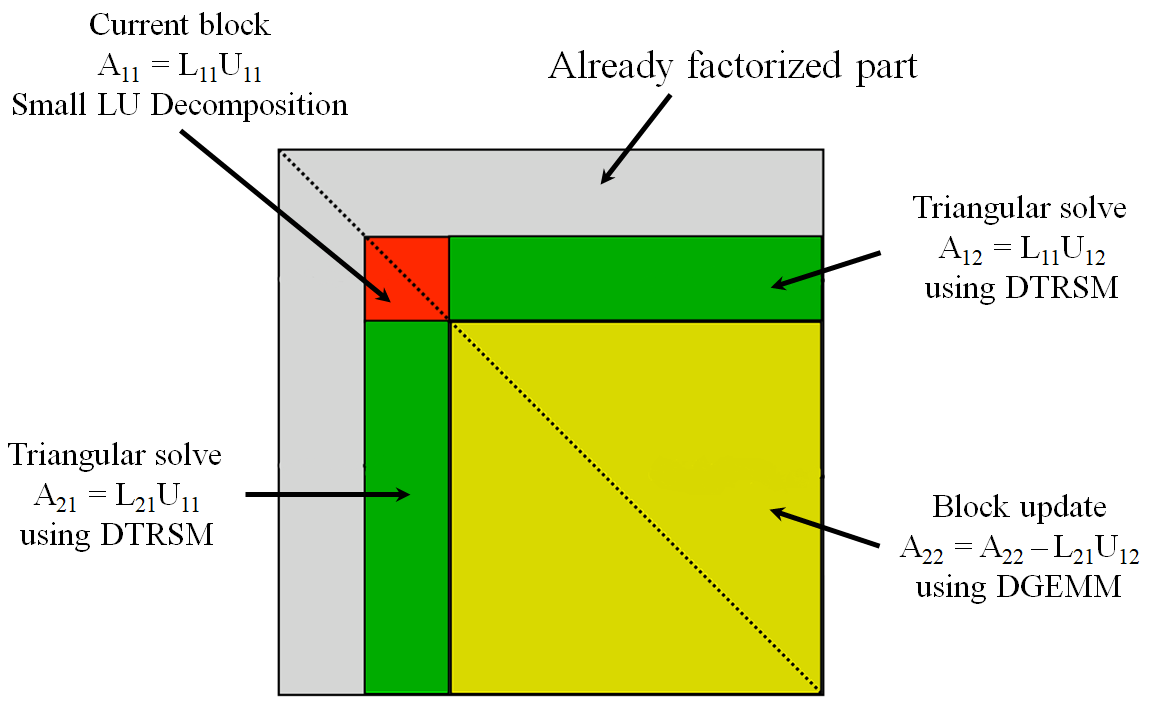
\includegraphics[width=0.75\textwidth]{figures/chapter-2/right-looking-la.png}
\caption{Right-looking parallel LU decomposition}
\label{fig:RightLookingLuReodering}
\end{figure}


% Show limited parallelism
It is clear the algorithm is purely sequential at the first steps when we compute small $LU$ decomposition. Therefore, it can have significant effect on algorithm strong scaling behavior. It should be mentioned that all three parallel implementations have the same problem i.e. they have an inherently sequential part at the beginning of a step. \\

Figure \ref{fig:lapack-lu-strong-scaling} shows results of strong scaling of dense $LU$ factorization performed for a couple of matrices filled with random numbers with different sizes: namely: $5000 \times 5000$, $10000 \times 10000$ and $15000 \times 15000$. LAPACK and OpenBLAS libraries were used for the test. One can easily notice that performance of dense $LU$ decomposition quickly deteriorates with reduction of the problem size. Additional factor that affects performance is strong scaling behavior of the triangular solve that we will discuss in section \ref{subseq:iterative methods}. 

\figpointer{\ref{fig:lapack-lu-strong-scaling}}
\begin{figure}[htpb]
  \centering
  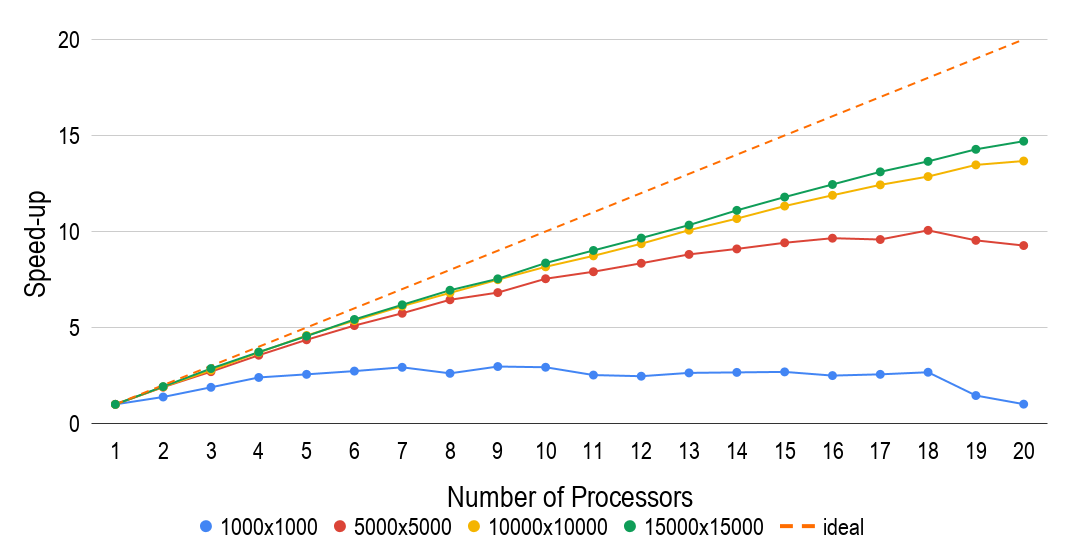
\includegraphics[width=0.85\textwidth]{figures/chapter-2/lapack-lu-strong-scaling.png}
\caption{Strong scaling of right-looking $LU$ decomposition using LAPACK and OpenBLAS}
\label{fig:lapack-lu-strong-scaling}
\end{figure}


\todo{add strong scaling for ScaLAPACK}
% results of strong scaling

Both left, right and Crout parallel matrix factorizations have been efficiently implemented in LAPACK (for shared-memory machines) and ScaLAPACK (distributed-memory machines) libraries. Both libraries belong to the Netlib project which is a repository of numerous scientific computing software maintained by AT\&T Bell Laboratories, the University of Tennessee, Oak Ridge National Laboratory and other scintific communities \cite{netlib-overview}. The libraries are built on top of Basic Linear Algebra Subprograms (BLAS) library. Figure \ref{fig:blas-lapack-scalapack} shows how these three libraries are coupled together.\\


\figpointer{\ref{fig:blas-lapack-scalapack}}
\begin{figure}[htpb]
  \centering
  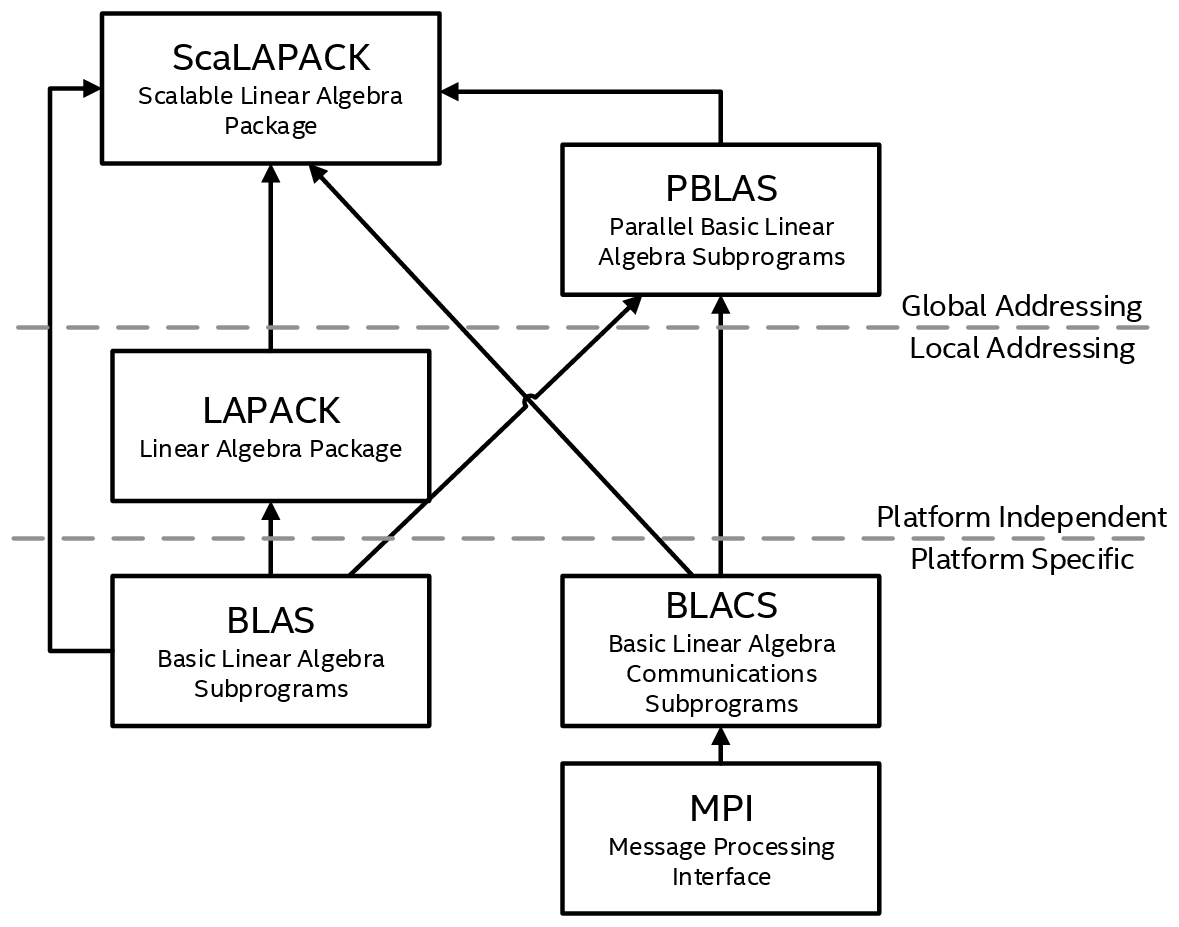
\includegraphics[width=0.65\textwidth]{figures/chapter-2/lapack-scalapack-blas.png}
\caption{A general view on BLAS, LAPACK and ScaLAPACK libraries \cite{netlib:lapack-scalapack-general-view}}
\label{fig:blas-lapack-scalapack}
\end{figure}

It is worth noting that BLAS can be considered as a foundation of LAPACK and ScaLAPACK libraries and, thus, it is the primary source of performance improvement. In particular we have to consider DGEMM, DTRSM BLAS subroutines performance because they, together with unblocked $LU$ factorization, compose the core of parallel $LU$ factorization algorithms as we discussed earlier.\\

There exist special-purpose, hardware-specific BLAS implementations developed by the hardware vendors i.e. IBM, Cray, Intel, AMD as well as open-source tuned implementations such as ATLAS, OpenBLAS, etc. We will come back to that discussion later and pay our close attention to a specific choice of a tuned BLAS library in subsection \ref{subseq:blas-comparison}.\\

In spite of all advantages of the direct dense solvers i.e. numerical stability and high ratio of floating point operations per memory access, we cannot consider this group of methods as a solver for time integration due to high complexity and storage costs.


\section{Iterative methods}
\label{subseq:iterative methods}
Iterative methods, especially Krylov subspace methods that we are going to discuss in this section, are well known for their relatively low storage requirements $O(nnz)$ and computation cost $O(N^2)$ in case of sparse linear systems of equations and good condition number. It turns out that sometimes it might be only one way to solve huge systems with millions unknowns.\\

The most well known methods are Conjugate Gradient (CG) for symmetric positive definite matrices, Minimal Residual Method (MINRES) for symmetric indefinite systems, Generalized Minimal Residual Method (GMRES) for non-symmetric systems of linear equations as well as different variants of GMRES such Biconjugate Gradient Method (BiCG), Biconjugate Gradient Stabilized Method (BiCGSTAB) and so on.\\

All Krylov methods solve a system of equation as a minimization problem. For example, the goal of CG algorithm is to minimize the energy functional $f(x) = 0.5 x^T A x - b^T x + c$, whereas, MINRES and GMRES tries to minimize residual norm $r_{j}$ for $x_{j}$ in a subspace. \\

%$j$th Krylov subspace $\mathcal{K}_{j}$. \\

The methods construct an approximate solution of a system as a linear combination of vectors $b$, $Ab$, $A^2b$, $A^3b$ and so on which defines the Krylov subspace. At each iteration we expand the subspace adding and evaluating a next vector in the combination.\\

Let's consider GMRES, as the most popular and general iterative solver, without preconditioning to just analyze its strong scaling behavior and potential problems. \\ 

As we mentioned above GMRES minimizes the residual norm in a subspace $U_m$.

\begin{equation} \label{eq:Gmres-1}
	\underset{x \in U_m}{min}||Ax - b||^2
\end{equation}

We can consider a solution vector $x$ in the subspace $U_m$ in a form $x=U_m y$. Thus, equation \ref{eq:Gmres-1} can be written as following:

\begin{equation} \label{eq:Gmres-2}
	\underset{x \in U_m}{min}||AU_m y - b||^2
\end{equation}

The most natural way to choose a proper subspace $U_m$ is the corresponding Krylov subspace $\mathcal{K}_m$ because it can be easily generated on the fly. However, decomposition of vector $x$ in that subspace can be a problem. Since the subspace $\mathcal{K}_m$ is spanned by the sequence of $b$, $Ab$, $A^2b$, ..., $A^{m-1}b$ and due to round-off error the sequence can become linear dependent. Therefore, we have to compute and use the orthonormal base of the given Krylov subspace. Saad and Schultz in their work \cite{sparse-la:gmrese-origin} used Arnoldi process for constructing an $l_2$-orthogonal basis. As the results equation \ref{eq:Gmres-2} can be written in the following form:  \\

\begin{equation} \label{eq:Gmres-3}
	\underset{x \in U_m}{min}||U_{m+1}H_{m+1,m} y - ||b||u_1||^2 = \\
	\underset{x \in U_m}{min}||H_{m+1,m} y - ||b||e_1||^2 
\end{equation}

where $H_m$ is an upper Hessenberg matrix. We can apply Givens rotation algorithm to compute $QR$ decomposition to convert $H_m$ to a strictly upper triangular matrix. Thus,

 
\begin{equation} \label{eq:Gmres-4}
	\underset{x \in K_m}{min}||Ax - b||^2 = \\
	\underset{x \in U_m}{min}||Q^TRy - ||b||e_1||^2 = \\
	\underset{x \in U_m}{min}||\Big(\begin{array}{c c}R_m \\ 0 \\\end{array}\Big) y - \Big(\begin{array}{c c} \tilde{b_m} \\ \tilde{b_{n-m}} \\\end{array}\Big)||^2
\end{equation}

Given \ref{eq:Gmres-4}, we can compute the solution as following:

\begin{equation} \label{eq:Gmres-5}
	R_m y = \tilde{b_m}
\end{equation}


\begin{equation} \label{eq:Gmres-6}
	x_m = U_m y  
\end{equation}

Because of large computational and storage costs, in case of evaluation of the full Krylov subspace, only small a subspace is computed, typically first 20 - 50 column vectors. Then the algorithm is restarted using the computed approximate solution as a initial guess for the next iteration.\\

We can see that some operations, for example \ref{eq:Gmres-6}, can be efficiently done in parallel. However, operatiopns like sparse triangular solve \ref{eq:Gmres-5} can introduce some effect on strong scaling behavior. Figure \ref{fig:sparse-triangular-solve-performance} shows strong scaling performance results of a sparse parallel triangular solver with a two dimensional matrix distribution. Performance considerations of the solver can be found in \cite{sparse-la:triangular-solve}.\\

\figpointer{\ref{fig:sparse-triangular-solve-performance}}

\begin{figure}[htpb]
  \centering
  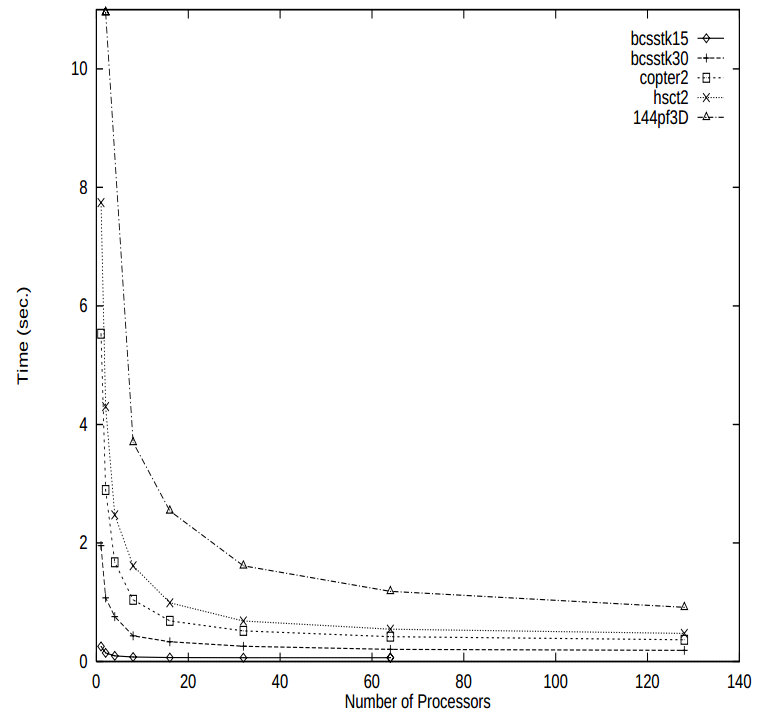
\includegraphics[width=0.5\textwidth]{figures/chapter-2/sparse-triangular-solve-performance.png}
\caption{Performance of sparse triangular solve \cite{sparse-la:triangular-solve}}
\label{fig:sparse-triangular-solve-performance}
\end{figure}


It is interesting to notice that performance of the triangular solver depends on a matrix sparsity structure as well as the matrix size. \\

Triangular solve \ref{eq:Gmres-5} can be computed in a single processor because matrix $R_m$ is usually small and depends on the number iterations before the restart. In this case the triangular solve can become a bottleneck again. \\

Figure \ref{fig:gmres-strong-scaling-speed-up} shows strong scaling performance results of the default GMRES solver from the PETSc library. The solver was set up without any preconditioner and 50 iterations as the restart. Additionally no stop criteria was specified except the maximum number iterations which was equal to 100. Four different matrices with different sparsity patterns were examined for the test. The information about the matrices is summarized in table \ref{table:matrix-info-1}. As we expected we can observe strong deviation of our test cases from the ideal speed-up when the number of processes exceeds 10.\\

It should be mentioned that parallelization overheads, introduced by such MPI operations as MPI\_Send, MPI\_Recv, MPI\_Allreduce, etc., also have their impact on performance of the algorithm.\\

\begin{table}[htpb]
\centering
\begin{tabular}{|c|c|c|c|}
\hline
Matrix Name & n       & nnz      & nnz / n \\ \hline
k3-18       & 1155955 & 7204723  & 6.2327  \\ \hline
k3-2        & 130101  & 13906057 & 6.0568  \\ \hline
cube-645    & 1000045 & 787997   & 13.9054 \\ \hline
cube-64     & 100657  & 1388993  & 13.7992 \\ \hline
\end{tabular}
\caption{Basic information about matrices used in figure \ref{fig:gmres-strong-scaling-speed-up}}
\label{table:matrix-info-1}
\end{table}

Other Krylov methods such as CG, for example, scales much better than GMRES. Because of the nature of the CG algorithm the next search direction can be found using a recurrent expression and the algorithms boils down to simple operations such as dot products and matrix vector multiplications. These operations can be easily parallelized and drop of performance comes only from MPI overheads. A quite comprehensive study about parallel CG algorithm performance can be found in \cite{sparse-la:cg}. The authors also introduced a deeply pipelined version of CG algorithm that scales even better due to overlapping the time-consuming global communication phase, induced by parallel dot product computations, with useful independent computations \cite{sparse-la:cg}.\\


\figpointer{\ref{fig:gmres-strong-scaling-speed-up}}
\begin{figure}[htpb]
  \centering
  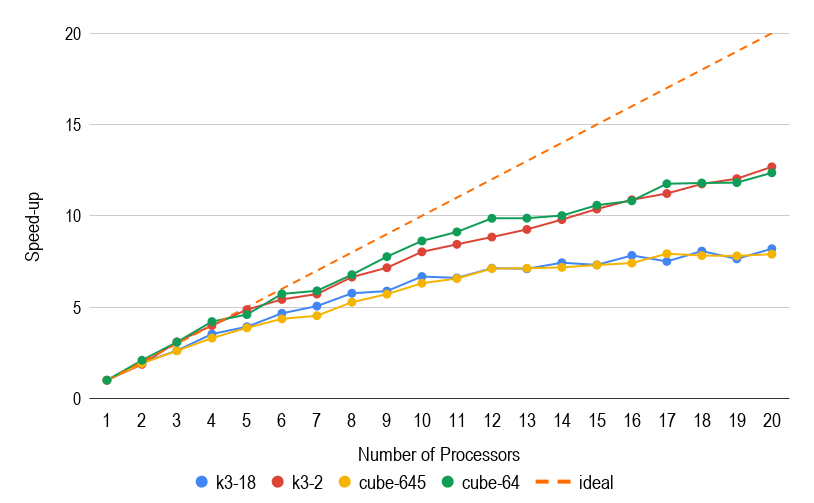
\includegraphics[width=0.8\textwidth]{figures/chapter-2/gmres-strong-scaling-speedup.png}
\caption{GMRES strong scaling speed-up}
\label{fig:gmres-strong-scaling-speed-up}
\end{figure}



% start discussion about preconditioning
The most important criteria of Krylov methods is convergence rate. The convergence rate of iterative methods strongly depends on a matrix and, in particular, on its condition number. For instance, equation \ref{eq:Gmres-7} shows dependence of the convergence rate from the matrix condition number. It can be clearly seen that a big condition number leads to very slow error reduction and, as the results, to huge number of iterations.\\

\begin{equation} \label{eq:Gmres-7}
	|| e^i ||_A \leq 2 ( \frac{\sqrt k - 1}{\sqrt k + 1} )^i || e^0 ||_A
\end{equation}

where $k = \frac{\lambda_{max}}{\lambda_{min}}$ - condition number of the corresponding matrix. \\

An obvious solution of such a problem is to reduce the condition number of the original system \ref{eq:slq}. A general method is to transform the original system in such a way that the conditional number of the transformed system gets significantly smaller. The transformation of \ref{eq:slq} can be done from the left side \ref{eq:pcn-1} or from the right one \ref{eq:pcn-2}.

\begin{equation} \label{eq:pcn-1}
	PAx = Pb
\end{equation}


\begin{equation} \label{eq:pcn-2}
	AP(P^{-1}x) = b
\end{equation}

where matrix $P$ is called preconditioner.\\


As an extreme example we can consider the inverse matrix $A^{-1}$ as the best preconditioner since it directly leads to the solution of the problem \ref{eq:slq} and, thus, it requires only one iteration. However, it is obvious that computation of inverse $A^{-1}$ is extremely expensive operation and it is not an objective of any iterative methods. That example helps understand and set requirements for preconditioners, namely:

\begin{enumerate}
	\item cheap to compute e.g. a 5-10 iterations of the corresponding Krylov solver
	\item should lead to a small conditioner number of the transposed system
	\item should be sparse, otherwise storage requirements will considerably increase
\end{enumerate}


There exist numerous techniques to compute preconditioners given a matrix $A$ e.g. (point) Jacobi, Block-Jacobi, incomplete $LU$ decomposition (ILU), multilevel ILU (ILU(p)), threshold ILU (ILUT), incomplete Cholesky factorization (IC), sparse approximate inverse (SPAI), multigrid as a preconditioner, etc. Almost all methods listed above have some tuning parameters which allow to get a better preconditioner i.e. a smaller condition number of the transformed system. However, it usually leads to increase of computational and storage costs. \\

Some methods can works particularly well for matrices derived from certain PDEs e.g. Poisson, Navier\-Stokes, etc. problems discretized using the cartesian grid. However sometimes it can take a considerable amount of time to choice right parameters for a certain preconditioning algorithm. It can become a challenge to fulfill all requirements 1, 2, 3 mentioned above. \\

Table \todo{Table with comparisons of different preconditioning for our test cases}

Table [] shows results of different preconditioning algorithms application to our test case. It can be seen that some algorithms failed even after tuning. \\

It interesting to notice that \citeauthor{wsmp} came to approximately the same results working on their set of matrices in their work \cite{wsmp}. They observed that preconditioned iterative solvers worked efficiently only for 2 out 5 cases in contrast to direct sparse solvers.\\

We can summarize that it is vital to perform careful parameter tuning of any preconditioning algorithms combining results from [table] and \cite{wsmp}. In general the  search can take a considerable amount of time. Moreover, it becomes impractical for time integration problems where topology of an underlying problem and, as the results, the computational mesh, discretization, Jacobian matrix can be changed over time of a simulation. It is obvious that parameters chosen for a particular time step can become not optimal for consecutive steps and, at the end, it can lead to divergence. If divergence happens at any time step the entire time integration algorithm fails and the simulation has to be restarted with different preconditioning parameters or with a different preconditioning algorithm.\\

By and large we come to a conclusion that preconditioned iterative solvers are not robust and thus cannot fully fulfill requirements listed in section \ref{chapter:solver configuration}.\\

% maybe above we have to mention inderect memory access and its effect on performance






\section{Direct sparse methods}
\label{subseq:sparse methods}
% it can be seen that it's easy to apply, however, it is not the case

% problems with a good preconditioner

% show motivation to use sparce direct methods: show a plot whith MUMPS and 100 interation of GMRES

% Give me the most popular sparce direct methods and compare them (goal: show that MUMPS it the most suitable package)

% Introduction to Multifrontal method: describe all three phases

% Parallelism for Multifrontal method: put stress on importance of elimination tree

% where and how we can exploid multi-threding

% show a result where multithreding works

% Choice of blas labraries
\section{Choice and Motivation}
\label{subseq:choice and motivation}



\section{Multifrontal Method}
\label{subseq:multifrontal method}

\section{Choice of BLAS library}
\label{subseq:blas-comparison}

